\documentclass[journal,12pt,twocolumn]{IEEEtran}
\usepackage{amsmath}
\usepackage{calc}
\usepackage{enumerate}
\usepackage{amssymb}
\usepackage{graphicx}
\usepackage{listings}
\lstset{
%language=C,
frame=single, 
breaklines=true,
columns=fullflexible
}


\title{PDF and CDF of uniform and gaussian distributions}
\author{Kushagra Gupta}

\date{}

\begin{document}

\maketitle

\section{Q 1.3}
\noindent Given $U$ is a uniformly distributed random variable over the interval $(0, 1)$, we have the density function $p_U(x)$:

\begin{align}
	p_U(x) =
            \begin{cases}
    		1, & x \in (0, 1) \\
    		0, & otherwise
	    \end{cases}
    	\label{eq:PDF}
\end{align}
%\begin{align}
%    &E(U) = \int _ {- \infty} ^ {\infty} {x d(F_u(x))} \\
%    &\int _ {- \infty} ^ {\infty} { d(F_u(x))} = 1
%\end{align}

We know that,
\begin{align}
    F_U(x) = \int_{-\infty}^{x} p_U(x) \,dx
    \label{eq:Relation}
\end{align}

\noindent $\therefore$ We have the following expression for $F_U(x)$:
\begin{align}
    F_U(x) =
	    \begin{cases}
	    	0, & x \in (-\infty, 0) \\
  	    	x, & x \in (0, 1) \\
    		1, & x \in (1, \infty)\\
            \end{cases}
\end{align}
\begin{align}
    \therefore d(F_U(x)) = 1 \times dx\\
\end{align}
\begin{align}
    \text{Now,}&E(U) = \int _ {-\infty} ^ {\infty} {x d(F_U(x))}\\
    \implies &E(U) = \int _ {0} ^ {1} {x dx}\\
    \implies &E(U) = 0.5
\end{align}

\begin{align}
    &E(U^1) = \int _ {- \infty} ^ {\infty} {x^2 d(F_u(x))} \\
    \implies &E(U^2) = \int _ {0} ^ {1} {x^2 dx} \\
    \therefore &E(U^2) = \frac{1}{3}
\end{align}

We know that
\begin{align}
    &var(U) = E(U^2) - (E(U))^2 \\
    \implies&var(U) = \frac{1}{3} - \frac{1}{4} \\
    \therefore &var(U) = \frac{1}{12} = 0.0825
\end{align}
\begin{figure}[!ht]
\centering
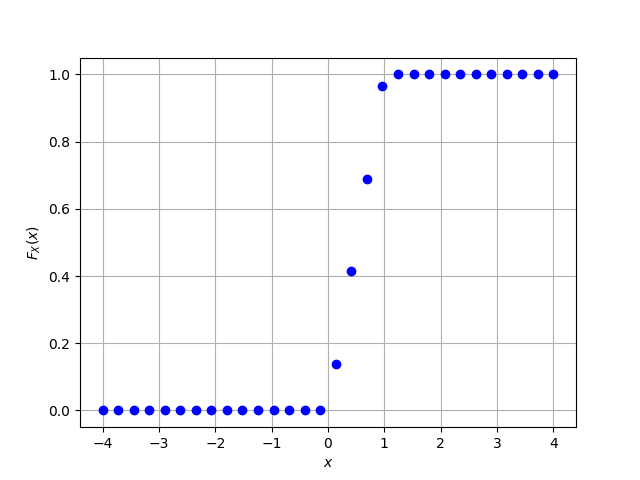
\includegraphics[width=\columnwidth]{./figs/Figure_Q1.png}
\caption{The CDF of $U$}
\label{fig: uniform distribution}
\end{figure}


    \begin{lstlisting}
        using ./code/exrand.c, we get the variance for the uniform distribution as 0.083301 and mean as 0.500007}
    \end{lstlisting}
\section {Q 1.5}
We are given that
\begin{align}
            &E[U^k] = \int^{\infty}_{-\infty} x^k dF_U(x)\\
    \implies&E[U^k] = \int^{\infty}_{-\infty} x^k p_U(x) \,dx		\label{eq: Expected}
\end{align}
We know that mean $\mu$ is given by $E(U)$.\\ Hence,

\begin{align}
    \mu &= \int_{-\infty}^{\infty} x p_U(x) \,dx\label{eq:Relation_1}\\
		\mu &= \int_{0}^{1} x \,dx \\
		&= \frac{x^2}{2} \big|^{1}_{0} \\
		&= \frac{1}{2} 	\label{eq: Mean}
\end{align}
\begin{align}
    var(U) = E((U - E(U))^2)
\end{align}
This can also be represented as
\begin{align}
		var(U) &= E(U^2 - 2E(U)U + (E(U))^2) \\
		&= E(U^2) - 2(E(U))^2 + (E(U))^2 \\
		&= E(U^2) - (E(U))^2
		\label{eq: Relation_2}
\end{align}
We can evaluate $E(U^2)$ using \eqref{eq: Expected} as:
	
\begin{align}
    	E(U^2) &= \int_{-\infty}^{\infty} x^2 p_U(x) \,dx \\
    	&= \int_{0}^{1} x^2 \,dx \\
    	&= \frac{x^3}{3} \big|^{1}_{0} \\
    	&= \frac{1}{3}
\end{align}

    Using \eqref{eq: Mean} and \eqref{eq: Relation_2} we have
\begin{align}
    	var(U) = \frac{1}{3} - \frac{1}{4} = \frac{1}{12}
\end{align}


\section{Q 2.2}
\begin{figure}[!ht]
\centering
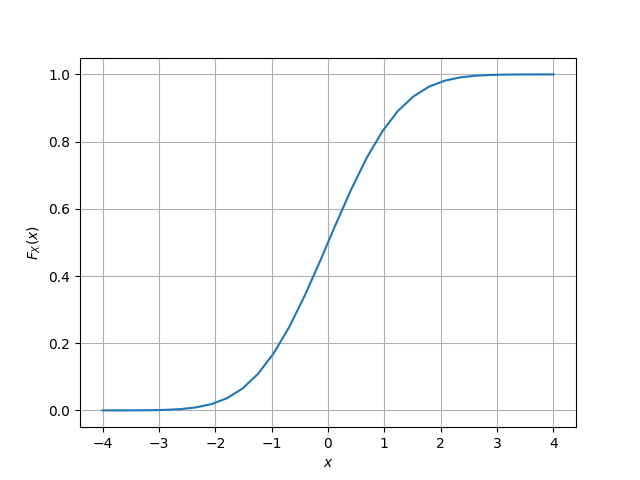
\includegraphics[width=\columnwidth]{./figs/Figure_2.png}
    \caption{The CDF of $X$}
\label{fig:gauss_X}
\end{figure}

\begin{figure}[!ht]
\centering
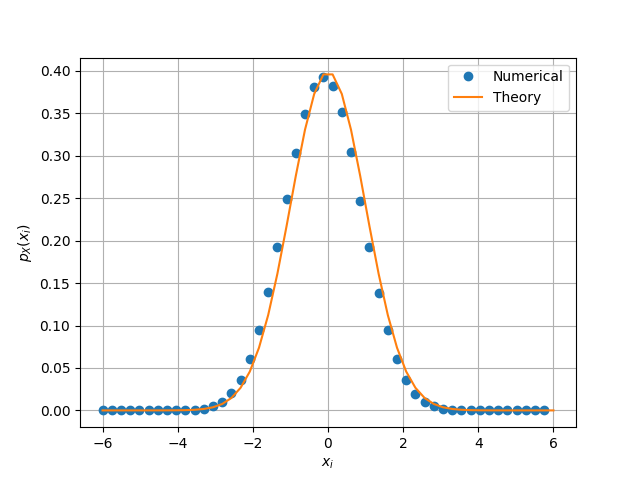
\includegraphics[width=\columnwidth]{./figs/Figure_3.png}
\caption{The PDF of $X$}
\label{fig:PDF_X}
\end{figure}

\section {Q 2.4}
\begin{lstlisting}
    using code ./code/exrand.c, we get the mean as 0.000326 and variance as 0.000906.
\end{lstlisting}


\section {Q 2.5}
\noindent For random variable $X$, we have been given the density function as follows
    \begin{align}
        &p_X(x) = \frac{1}{\sqrt{2\pi}}\exp{\frac{-x^2}{2}}\\
    \end{align}
For finding $\mu$,
\begin{align}
    \mu &= \int _ {- \infty} ^ {\infty} {x . p_X(x) dx} \\
    &= \int _ {- \infty} ^ {\infty} {x . \frac{1}{\sqrt{2 \pi}} e^{-x^2 / 2} dx}
\end{align}

As $x . p_X(x)$ is an odd function the above integral is $0$, therefore $\mu = 0$

For finding the variance $var$,
\begin{align}
    var &= E(X^2) \\
    &= \int _ {- \infty} ^ {\infty} {x^2 . \frac{1}{\sqrt{2 \pi}} e^{-x^2 / 2} dx} \\
    \text{let\,\,} x^2 &= 2t \\
    \implies var &= \int _ {- \infty} ^ {\infty} {\sqrt{2t} . \frac{1}{\sqrt{2\pi}} e^{-t} dt} \\
    &= \frac{2}{\sqrt{\pi}} \Gamma \left(\frac{3}{2}\right) \\
    \implies var &= 1
\end{align}
\section{Q 3.2}
We have been given that random variable $V$ is a function of the random variable $U$ as follows:
\begin{align}
    V = -2\ln{(1 - U)}
\end{align}
	Note that the obtained distribution function (CDF) for random variable $U$ is:
\begin{align}
    	F_U(x) =
	\begin{cases}
		0, & x \in (-\infty, 0) \\
		x, & x \in (0, 1) \\
		1, & x \in (1, \infty)
	\end{cases}
\end{align}
We know for any random variable $X$
\begin{align}
    F_X(x) = \Pr(X \leq x)
\end{align}
	Hence, we can write:
\begin{align}
	F_V(x) &= \Pr(V \leq x) \\
	&= \Pr(-2\ln{(1 - U)} \leq x)\\
	&= \Pr(U \leq 1 - \exp{\frac{-x}{2}})\\
	&= F_U(1 - \exp{\frac{-x}{2}})
\end{align}
Note that the function $f(x) = 1 - \exp{\frac{-x}{2}}$ follows:
\begin{align}
    f(x) \in
	\begin{cases}
	    {0}, & x \in (-\infty, 0) \\
	    (0, 1) & x \in (0, \infty)
	\end{cases}
\end{align}
Hence we can write
\begin{align}
	F_V(x) =
	\begin{cases}
	    0, & x \in (-\infty, 0) \\
	    1 - \exp{\frac{-x}{2}}, & x \in (0, \infty)
    	\end{cases}
\end{align}
\begin{figure}[!ht]
\centering
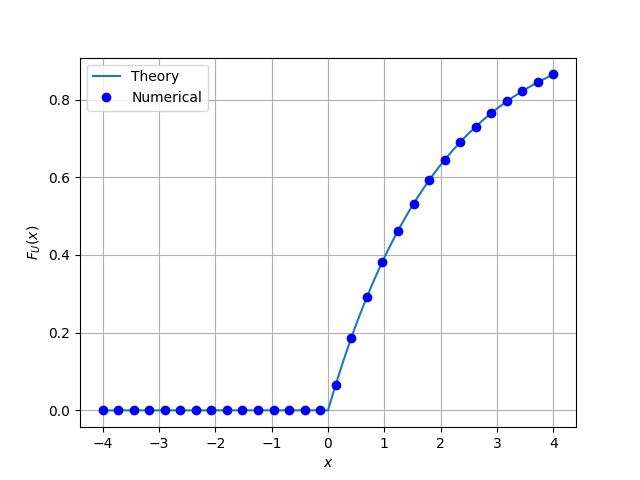
\includegraphics[width=\columnwidth]{./figs/Figure_Q4.png}
\caption{The CDF of $V$}
\label{fig:CDF_V}
\end{figure}









\end{document}
